\chapter{Background}\label{chapter:background}
Currently, state-of-the-art models in machine learning often perform best when using a pre-trained backbone. These backbones are trained on well-known public datasets, such as ImageNet~\cite{deng2009imagenet} for image-related tasks or Common Crawl~\cite{commoncrawl} for text-based tasks. These pre-trained backbones or foundation models, are then used for fine-tuning on specific tasks. The benefits, and risks, are described in great detail by Bommasani et al.~\cite{DBLP:journals/corr/abs-2108-07258}. A few will be highlighted here.

The main benefits of using pre-trained networks are two-fold: they typically improve the convergence speed of the model and reduce the amount of task-specific data required~\cite{donahue2014decaf,zeiler2014visualizing}. Furthermore, many of the state-of-the-art models in various (image) related tasks, such as object detection~\cite{liu2016ssd,redmon2016you} and semantic segmentation~\cite{orsic2019defense,girshick2014rich} benefit from pre-trained backbones.

A drawback of these generic datasets is that, in many real-world robotic applications, the actual data distribution encountered is a tiny subset of those seen during training. Thus the question arises; does a robot tasked with navigating an indoor warehouse benefit from knowing how to detect an elephant or other (big) animals? This is specifically the case with mobile robotics where computational resources are scarce. Thus by pre-training on the actual dataset, could it avoid learning these useless parts and thereby possibly increase the accuracy on the task at hand? However, these task-specific datasets are often non-existent, and although collecting task-relevant data can often easily be done, e.g. by collecting videos of a warehouse by manually driving a robot around for a day, it remains expensive to convert this raw data into a useful dataset due to the labour required to \emph{properly} label it.
In their systematic review of ImageNet, Mishkin et al.~\cite{MISHKIN201711}, show that a smaller high-quality dataset results in better performance compared to a larger low-quality dataset. Therefore, it would be ideal if we could learn most of the important features from the raw data, i.e. unsupervised learning.

\section{Variational Auto-Encoder}
A Variational Auto-Encoder (VAE) is a model that can be trained purely on images without requiring any manual labelling. The concept of the VAE was independently proposed by Kingma et al.~\cite{kingma2014autoencodingvariationalbayes} and Rezende et al.~\cite{rezende2014stochastic}. The general idea behind the VAE is that there is a complex parametrizable distribution $p_\theta(x)$ of interest. Understanding the parameters allows us to either deepen the understanding of the process by which samples of $x$ are generated or to allow us to mimic the natural data. It is assumed that the distribution is the result of a process involving some prior distribution $p_\theta(z)$. First, a value $z$ is generated by $p_\theta(z)$, after which $x$ is generated from the conditional distribution $p_\theta(x | z)$, which together can be modelled as $p_\theta(x, z) = p_\theta(x|z)p_\theta(z) = p_\theta(z|x)p_\theta(x)$. The VAE proposes to approximate the conditional distribution, $p_\theta(z|x)$, using an \emph{encoder} model $q_\phi(z|x)$. The marginal log-likelihood can be described by Eq.~\ref{eq:marginal_likelihood} and as the Kullback-Leibler (KL) Divergence~\cite{kullback1951information} is $\geq 0$, the remaining term is the lower bound of the marginal log-likelihood. The remaining term can be further rewritten into Eq.~\ref{eq:elbo}.
\begin{subequations}
    \begin{align}
        \log p_\theta(x)   & = \mathbb{E}_{q_{\phi}(z|x)}[-\log q_\phi(z|x) + \log p(x,z)] + D_{KL}(q_{\phi}(z|x) || p_\theta(z|x))\label{eq:marginal_likelihood} \\
        \log p_\theta(x)   & \geq \mathbb{E}_{q_{\phi}(z|x)}[-\log q_\phi(z|x) + \log p(x,z)] = \mathcal{L}_{ELBO}                                                \\
        \mathcal{L}_{ELBO} & = \mathbb{E}_{q_{\phi}(z|x)}[\log p_\theta(x|z)] - D_{KL}(q_{\phi}(z|x) || p_\theta(z))\label{eq:elbo}
    \end{align}
\end{subequations}
This lower bound can then be optimized w.r.t. to our parameters using gradient optimization. By choosing a prior $p_\theta(z)$ for which the KL divergence can be integrated analytically, we only need to approximate the reconstruction error $\mathbb{E}_{q_{\phi}(z|x)}[\log p(x|z)]$ using sampling. Empirically, Kingma et al. found that when the batch size is large enough, a single sample per image is enough. This allows us to efficiently optimize the VAE's parameters and reduce the computational complexity of training. The last hurdle to approximating the distributions $q_{\phi}(z | x)$ and $p_{\theta}(x | z)$ with neural networks is that distributions are not differentiable. However, this can be circumvented using the reparametrization trick. A differentiable transformation $f_\phi(x, \epsilon)$. $\epsilon$ is drawn from a random distribution $p(\epsilon)$. An example of the Gaussian is shown in Eq.~\ref{eq:reparametrization-trick}. This can easily be extended to a broad range of distributions.
\begin{equation}
    \begin{split}
        \mu, \sigma & = f_\phi(x)                     \\
        \epsilon    & \sim \mathcal{N}(0, 1)          \\
        z           & = \mu + \sigma^2 \cdot \epsilon
    \end{split}
    \label{eq:reparametrization-trick}
\end{equation}
However, there exist a few problems with VAEs~\cite{tomczak2021deep}, e.g. \emph{blurry samples} (see Appendix~\ref{appendix:recon_samples}), \emph{posterior collapse}~\cite{DBLP:journals/corr/BowmanVVDJB15}, and the fact that the latent space is not necessarily `disentangled'~\cite{higgins2017betavae}. A latent space that is properly disentangled will have ideally one latent unit being responsible for one aspect of the generative process. This means that changing that unit results in a single (semantic) change in the generated sample. In the case of face generation, this could for example be the shape of the nose or the colour of the skin. Properly disentangled latent spaces make it easier to fine-tune models on subsequent tasks~\cite{bengio2014representationlearningreviewnew}, and are therefore of paramount importance to us. The $\beta$-VAE, proposed by Higgins et al.~\cite{higgins2017betavae}, multiplies the KL divergence with a hyperparameter $\beta$, resulting in Eq.~\ref{eq:beta-elbo}. If this value is set to 1, it results in a standard VAE. In their paper, they show that for $\beta$-values greater than 1, the learnt latent representation is more disentangled. Note, that there is no additional information required about the data for this to be learnt. By increasing the $\beta$, the capacity of the latent space is reduced. This means that less information can be passed due to the stronger regularization force of the KL-divergence.
\begin{equation}
    \mathcal{L}_{\beta-ELBO} = \mathbb{E}_{q_{\phi}(z|x)}[\log p(x|z)] - \beta \cdot D_{KL}(q_{\phi}(z|x) || p(z))
    \label{eq:beta-elbo}
\end{equation}
However, when the $\beta$ is too large, it will result in a posterior collapse. This is because the model is strongly incentivized to ensure that the posterior is equal to the prior.

There exist many more extensions to the classical VAE, most of which can be divided into one of the following four categories.

\emph{Better encoders}, such as flow-based models~\cite{Berg2018SylvesterNF,tomczak2017improving,rezende2015variational}. \emph{Better priors}, such as VampPrior~\cite{tomczak2018vae} in which the prior is a mixture of Gaussians, with additional pseudo-inputs learnt from the training data to prevent overfitting. \emph{Better decoders}, such as transformer-based decoders~\cite{Henderson2022AVA,9054554} and lastly, \emph{Hierarchical-VAEs} (HVAE), of which the most notable are the Ladder-VAE~\cite{NIPS2016_6ae07dcb}, the BIVA~\cite{maaloe2019biva} and NVAE~\cite{vahdat2020nvae}. These models extract a latent space from multiple levels of the encoder. During the generation phase, these latent variables are then generated based on the decoder. Compared to classic-VAEs they are capable of generating far sharper images. However, they are more complicated to train and often consist of more parameters. Thereby, resulting in a slower inference.


\section{Semantic Slam}
Simultaneous Localization and Mapping (SLAM)~\cite{chatila1985position} is a powerful method used for the automated navigation of robotic vehicles. It is capable of simultaneously creating a map of an unknown environment and navigating that same environment. This is a vital part of autonomous robotic vehicles. With the rise of deep learning methods in computer vision, many visual-based SLAM algorithms have been created~\cite{taketomi2017visual}. More recent algorithms use semantic segmentation networks, such as DS-SLAM~\cite{yu2018ds}. DS-SLAM uses SegNet~\cite{badri2017segnet} to extract the semantic information from images. By improving the quality of this model, the complete system would become more stable.

\subsection{Semantic segmentation}
Semantic segmentation is a computer vision technique that involves assigning a label or category to each pixel in an image. This means that, rather than just detecting objects, the method also identifies what those objects are (e.g.\,chair, person, road) and is able to provide an exact contour of the object. The goal of semantic segmentation is to produce a dense prediction map that classifies every pixel in the image into one of the predefined categories.

One of the first more successful deep learning methods for semantic segmentation was the Fully Convolutional Network (FCN) proposed by Long et al.~\cite{long2015fully}. Which was slightly improved by Ronneberger et al.~\cite{ronneberger2015u}, and named U-Net, referencing the shape of the model. The architecture of the model can be seen in Figure~\ref{fig:unet-architecture}. Due to the structure, the output can take both fine-grained information, which is useful to have good localization, and global information, which improves the classification. This method is robust and reliable, making it easy to train and use in real-time applications.
\begin{figure}[ht]
    \centering
    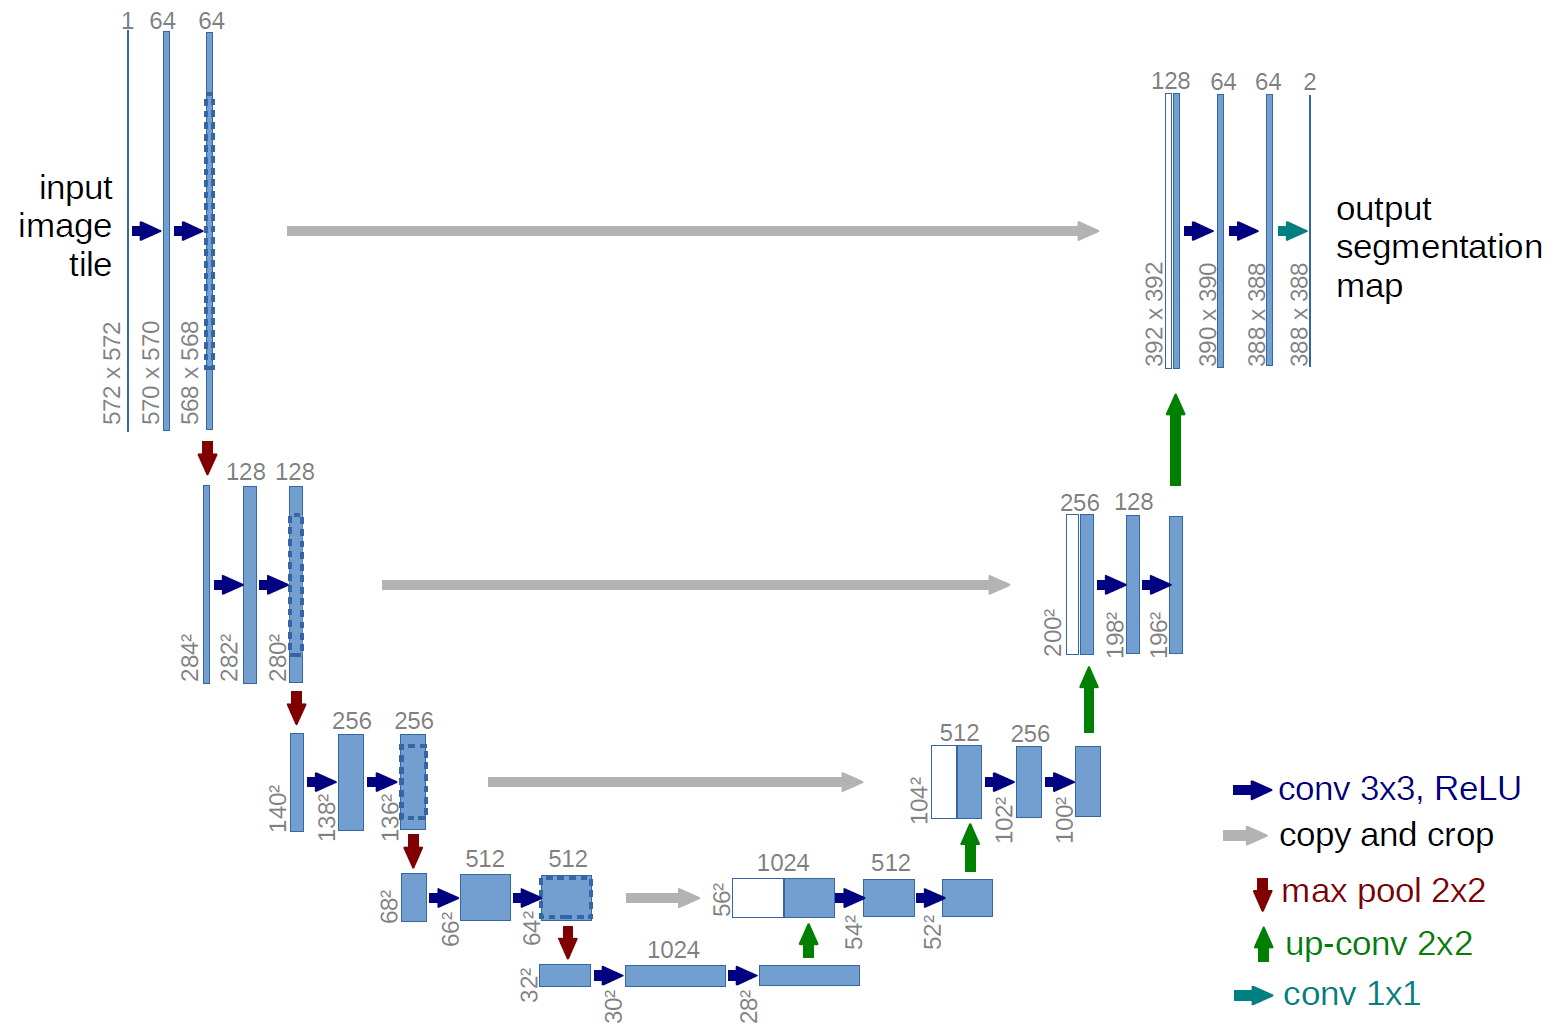
\includegraphics[width=0.5\textwidth]{figures/unet-architecture.png}
    \caption{U-Net Architecture~\cite{ronneberger2015u}}
    \label{fig:unet-architecture}
\end{figure}

The Feature Pyramid Network (FPN)~\cite{lin2017feature} shares part of its structure with the U-Net, except it explicitly combines the features of each upscaling layer to predict the final semantic segmentation mask as visualized in Figure~\ref{fig:fpn-architecture}. The main difference between FPN and U-Net is that FPN takes more time to process images. It does produce better results for smaller and medium-sized objects.

\begin{figure}[ht]
    \centering
    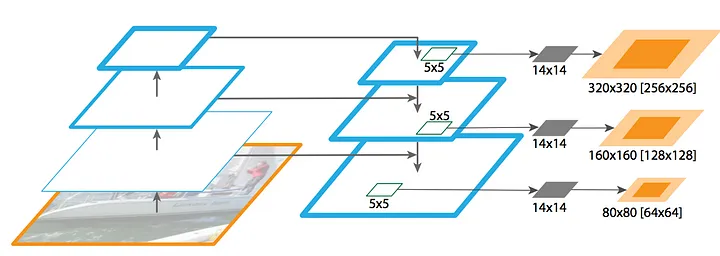
\includegraphics[width=0.5\textwidth]{figures/fpn-architecture.png}
    \caption{Feature Pyramid Network Architecture~\cite{lin2017feature}}
    \label{fig:fpn-architecture}
\end{figure}

These models are very adaptable as their various parts, such as encoders, can easily be replaced. Thus, they can be modified to adapt to the limitations of mobile robotics, by employing lightweight and fast encoders. Moreover, during the BRaTS2018~\cite{menze2014multimodal} competition, it has been shown that a simple U-Net can be very competitive. It achieved second place~\cite{DBLP:journals/corr/abs-1809-10483} during the competition. Next to that, they also both employ an encoder-decoder structure, which is similar to the VAE. Thus resulting in a more representative comparison. Furthermore, they are simple to get working and do not require any exotic tricks to achieve usable results.
